\documentclass[aspectratio=169]{beamer}
%
% Choose how your presentation looks.
%
% For more themes, color themes and font themes, see:
% http://deic.uab.es/~iblanes/beamer_gallery/index_by_theme.html
%
\mode<presentation>
{
    \usetheme{default}      % or try Darmstadt, Madrid, Warsaw, ...
    \usecolortheme{default} % or try albatross, beaver, crane, ...
    \usefonttheme{default}  % or try serif, structurebold, ...
    \setbeamertemplate{navigation symbols}{}
    \setbeamertemplate{caption}[numbered]
}

\usepackage[english]{babel}
\usepackage[utf8]{inputenc}
\usepackage{graphicx}
\usepackage{breqn}
\usepackage{bbm}
\usepackage{multicol}
%\usepackage{enumitem}

\newenvironment{wideitemize}{\itemize\addtolength{\itemsep}{10pt}}{\enditemize}

\DeclareMathOperator*{\argmax}{arg\,max}
\DeclareMathOperator*{\argmin}{arg\,min}

\usepackage[style=authoryear, backend=biber]{biblatex}
\addbibresource{}

\title{A Null Effect of Government Shutdowns on Bureaucrat Selection}
\author{Nathaniel Bechhofer \and Churn Ken Lee}
\institute{UC San Diego}
\date{}

\begin{document}

\begin{frame}
    \titlepage
\end{frame}

\begin{frame}
    \frametitle{Question}

    Is there negative selection due to shutdowns and furloughs?

\end{frame}

\begin{frame}
    \frametitle{Why do we care?}

    \begin{wideitemize}
        \item Government shutdowns are an important part of how the US government negotiates budgeting in the modern partisan era
        \item Wider literature in both low  and high income countries indicates importance of government worker quality for delivery of services
        \item Shutdowns may be costly in the long run by pushing talented workers out of the government
        \begin{figure}[]
            \centering
            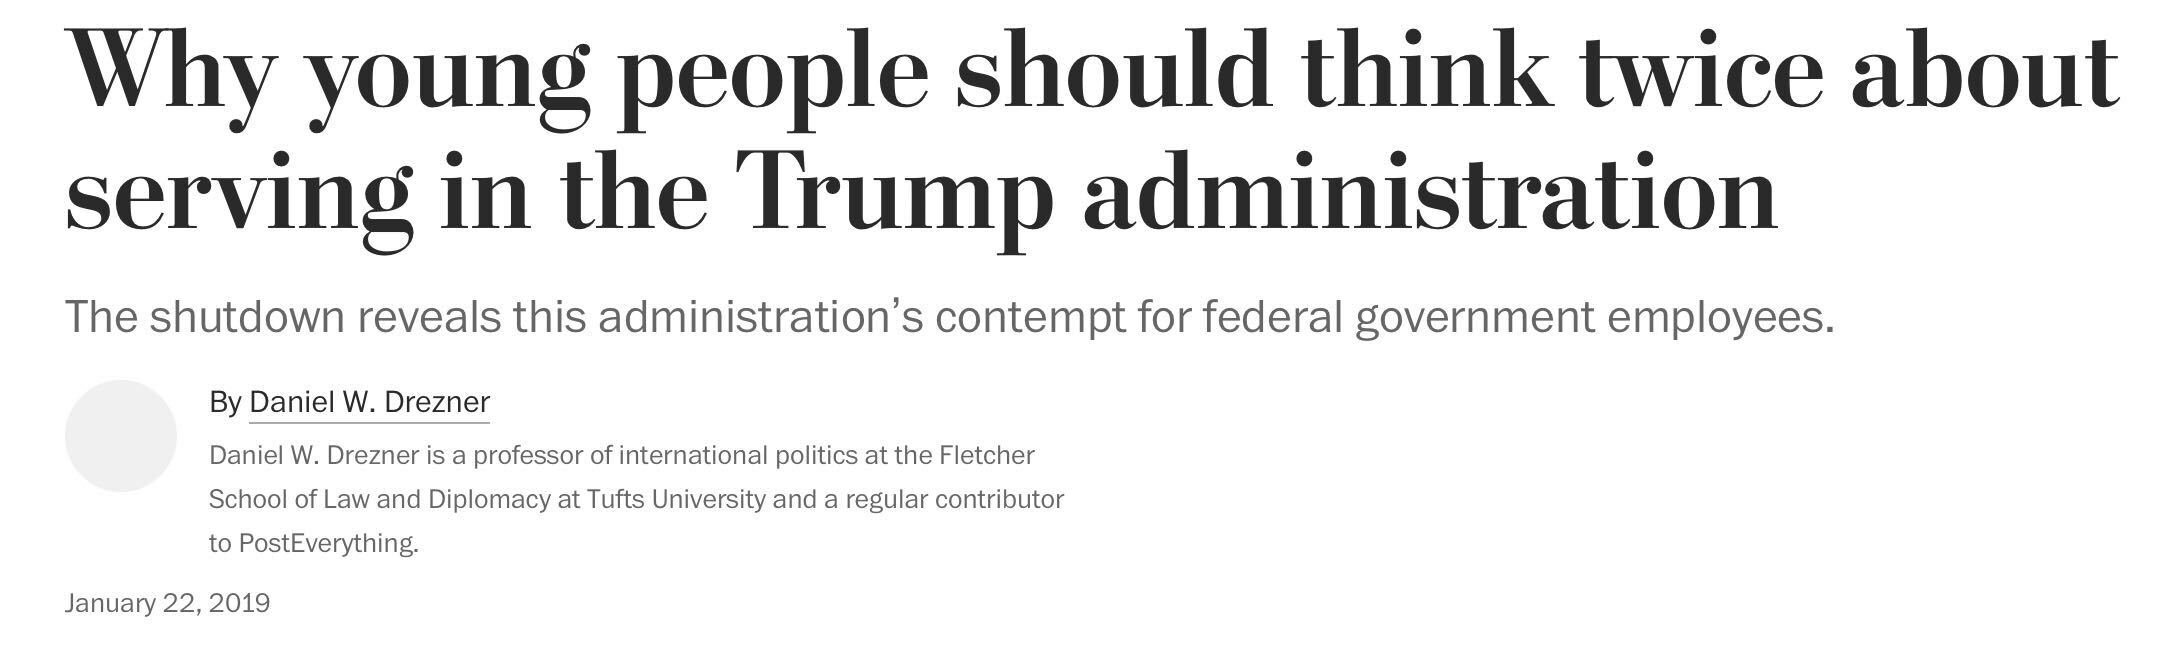
\includegraphics[width=0.5\textwidth]{../output/image_from_ios.jpg}
        \end{figure}
        \item If this cost is minimal, government shutdowns may be a decent institutional arrangement to ensure agreements over budgeting given the constraints of current partisanship
    \end{wideitemize}

\end{frame}

\begin{frame}
    \frametitle{Data}

    \begin{wideitemize}
        \item Buzzfeed News FOIA payroll data for federal government employees
        \item Employees from 1973 onwards
        \item Occupation, pay, tenure, (some) demographic information
        \item Flows since 1982
        \item Data since 2014 has employee ID withheld, so matching after 2014 using ID is not possible
        \item We use non-DoD personnel
    \end{wideitemize}

\end{frame}

\begin{frame}
    \frametitle{Variables available in status files}

    \begin{multicols}{2}
        \begin{itemize}
            \item Pseudo ID
            \item Name (redacted for some)
            \item Date
            \item Agency
            \item Location (redacted for some)
            \item Age
            \item Years since degree
            \item Education level
            \item Pay plan
            \item Pay grade
            \item Tenure (in ranges)
            \item Occupation
            \item Occupation category (broad)
            \item Pay
            \item Supervisory status
            \item Type of appointment
            \item Work schedule
        \end{itemize}
    \end{multicols}

\end{frame}

\begin{frame}
    \frametitle{Variables available in dynamics files}

    \begin{multicols}{2}
        \begin{itemize}
            \item Pseudo ID
            \item Name (redacted for some)
            \item Agency
            \item Accession/separation indicator (reason available after 1987)
            \item date
            \item Age
            \item Pay plan
            \item Pay grade
            \item Tenure
            \item Location
            \item Occupation
            \item Occupational category
            \item Pay
            \item Type of appointment
            \item Work schedule
        \end{itemize}
    \end{multicols}

\end{frame}

\begin{frame}
    \frametitle{Aggregate separation rates}

    \begin{figure}[]
        \centering
        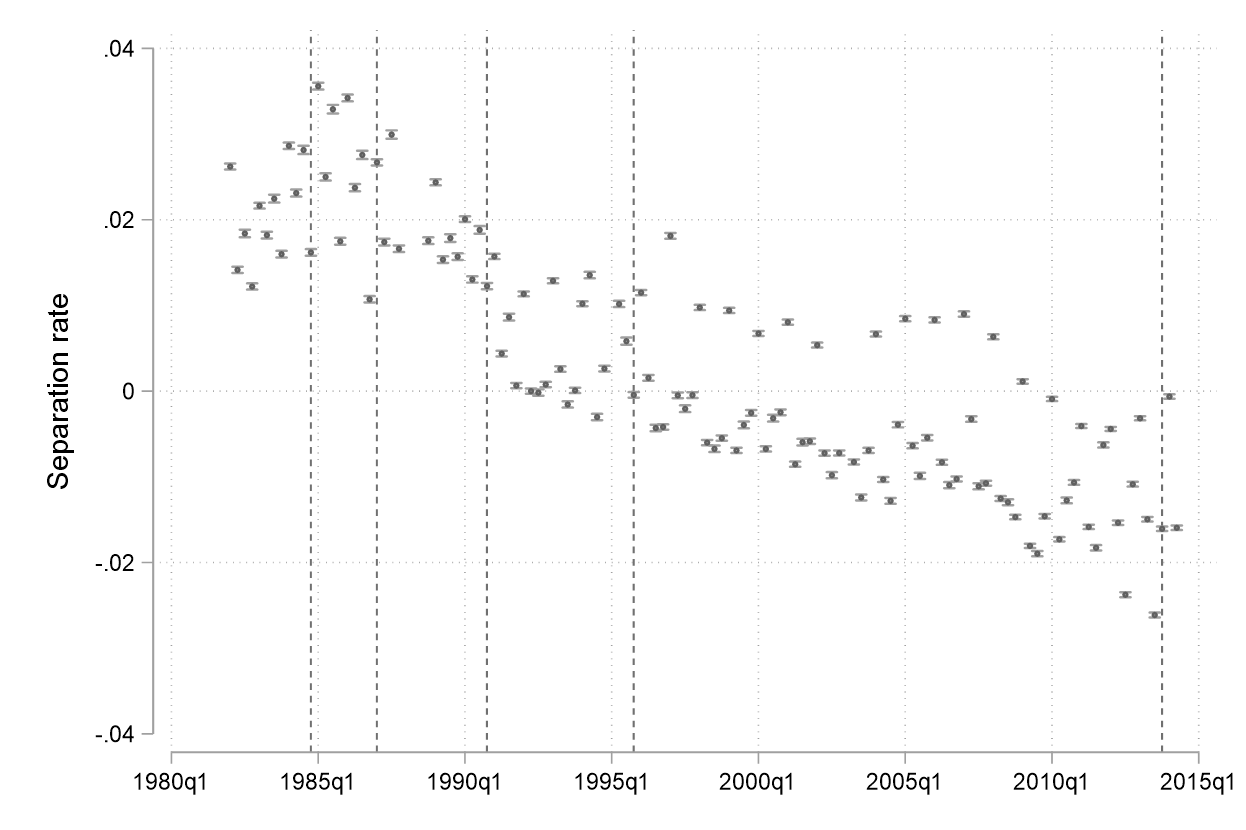
\includegraphics[width=0.9\textwidth]{../output/separation_rate_adj_CI.png}
    \end{figure}

\end{frame}

\begin{frame}
    \frametitle{Aggregate entry rates}

    \begin{figure}[]
        \centering
        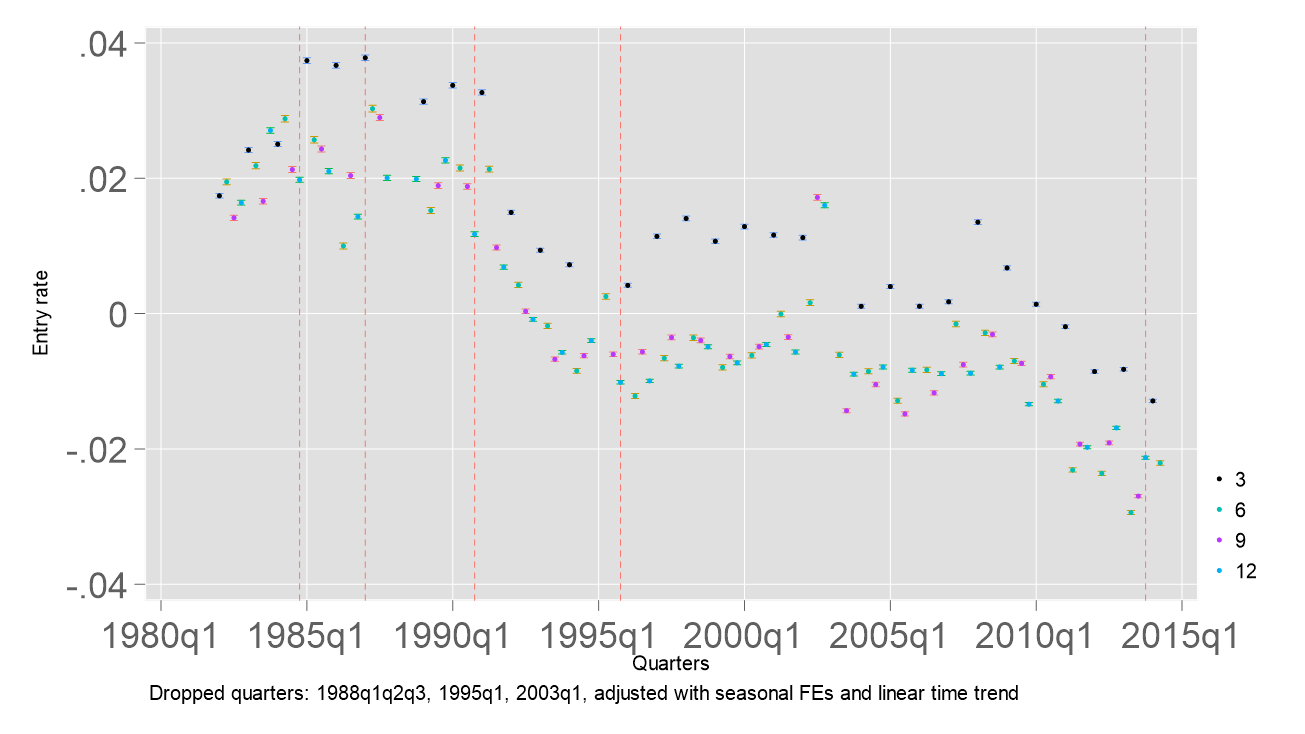
\includegraphics[width=0.9\textwidth]{../output/accession_rate_adj_CI.png}
    \end{figure}

\end{frame}

\begin{frame}
    \frametitle{Event study: high vs low education separation rates}

    \begin{figure}[]
        \centering
        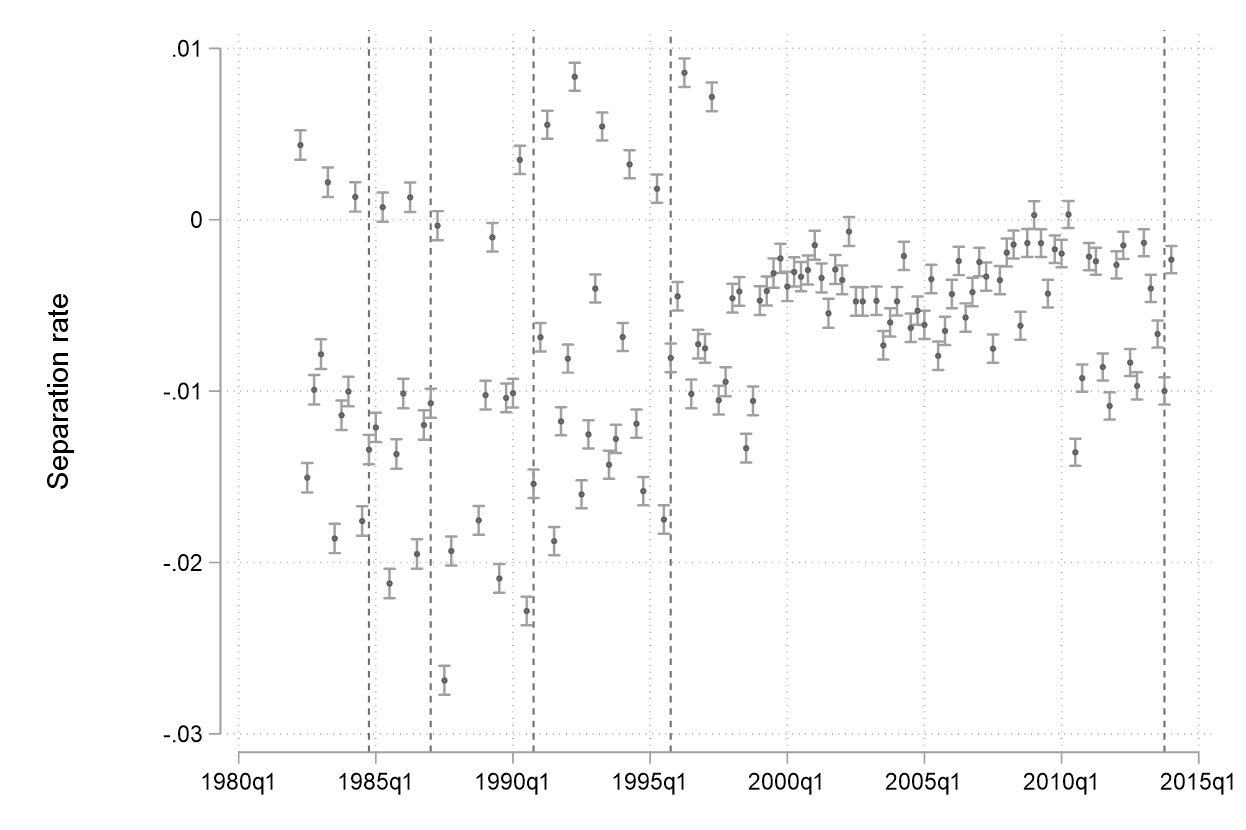
\includegraphics[width=0.9\textwidth]{../output/separation_rate_educ.png}
    \end{figure}

\end{frame}

\begin{frame}
    \frametitle{Event study: high vs low education entry rates}

    \begin{figure}[]
        \centering
        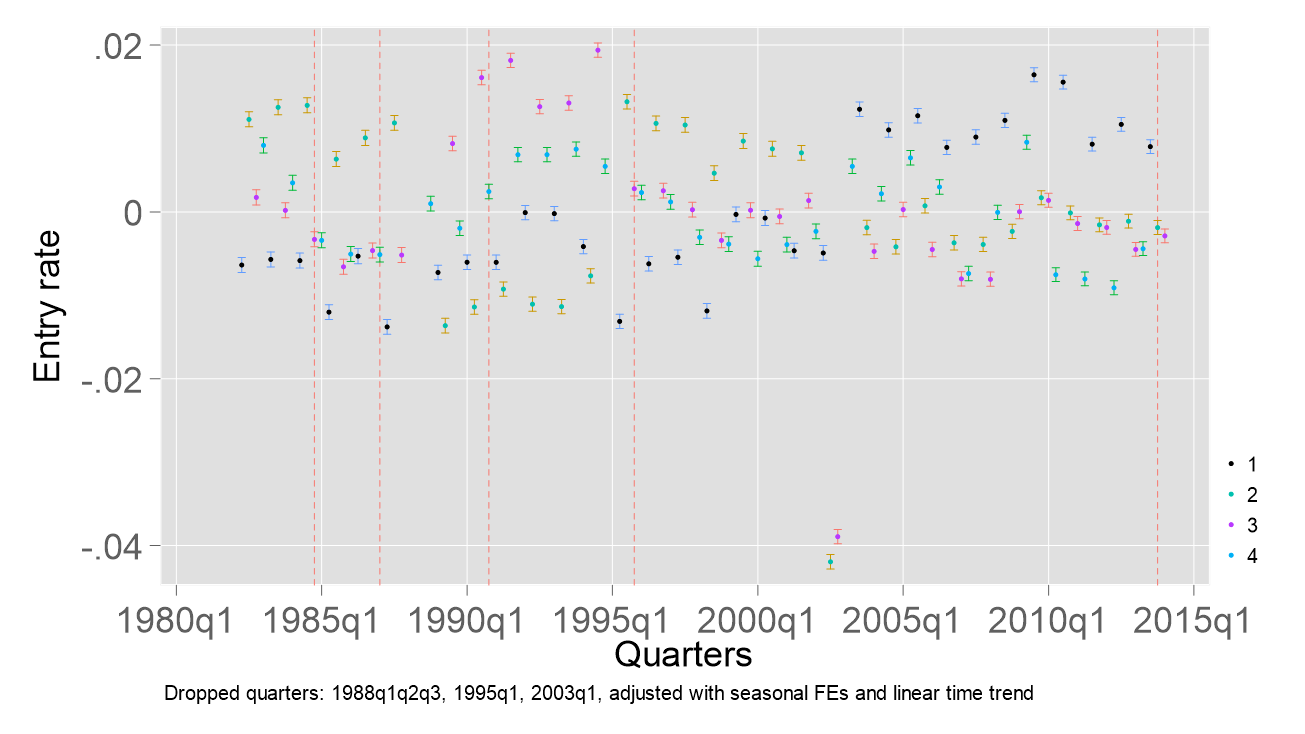
\includegraphics[width=0.9\textwidth]{../output/accession_rate_educ.png}
    \end{figure}

\end{frame}

\begin{frame}
    \frametitle{Event study: high vs low pay separation rates}

    \begin{figure}[]
        \centering
        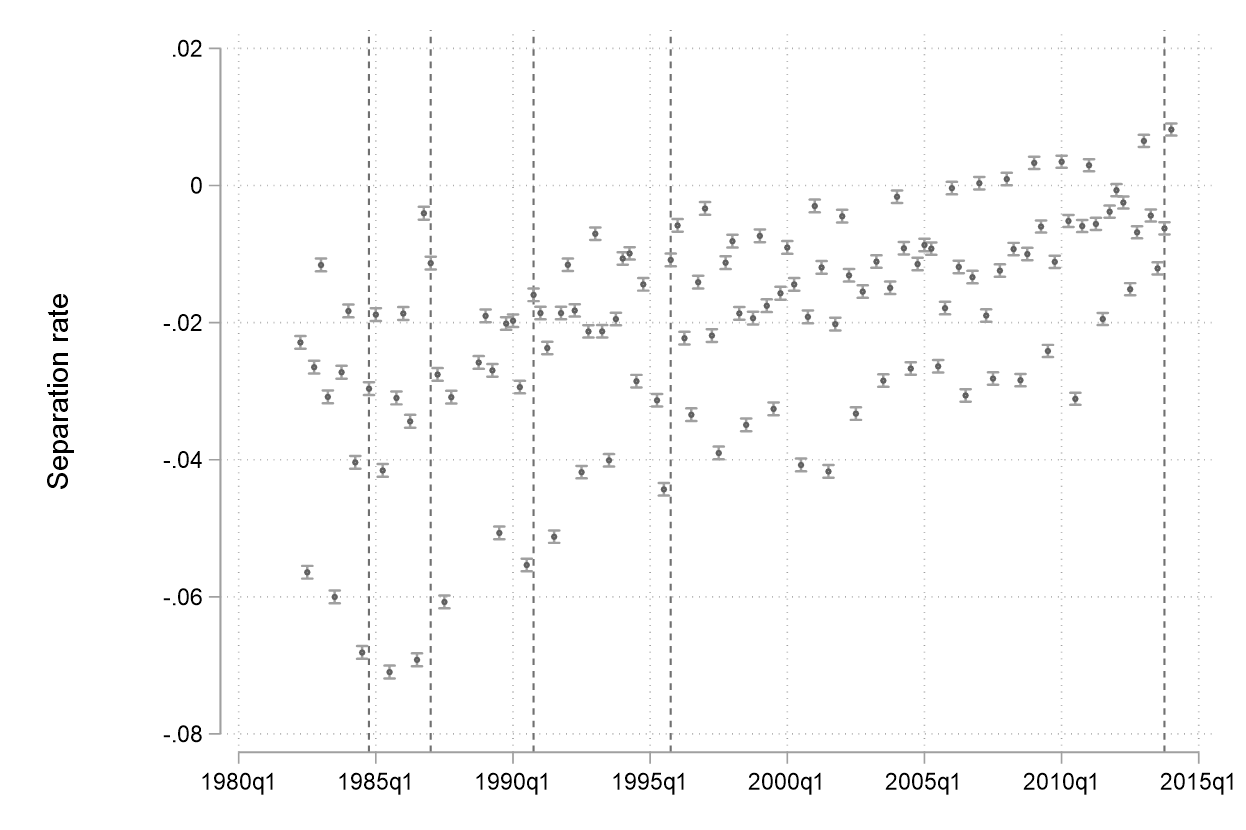
\includegraphics[width=0.9\textwidth]{../output/separation_rate_med_pay.png}
    \end{figure}

\end{frame}

\begin{frame}
    \frametitle{Event study: high vs low pay entry rates}

    \begin{figure}[]
        \centering
        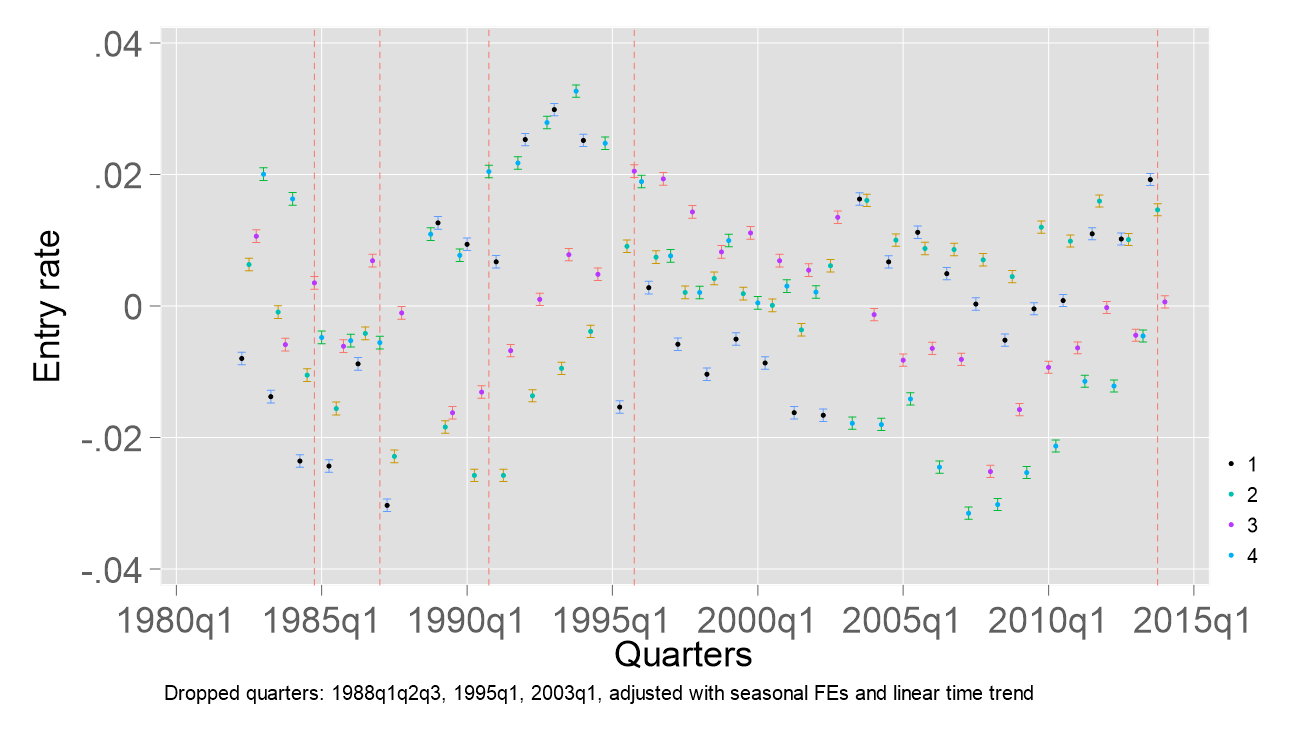
\includegraphics[width=0.9\textwidth]{../output/accession_rate_med_pay.png}
    \end{figure}

\end{frame}

\begin{frame}
    \frametitle{Event study: high vs low tenure separation rates}

    \begin{figure}[]
        \centering
        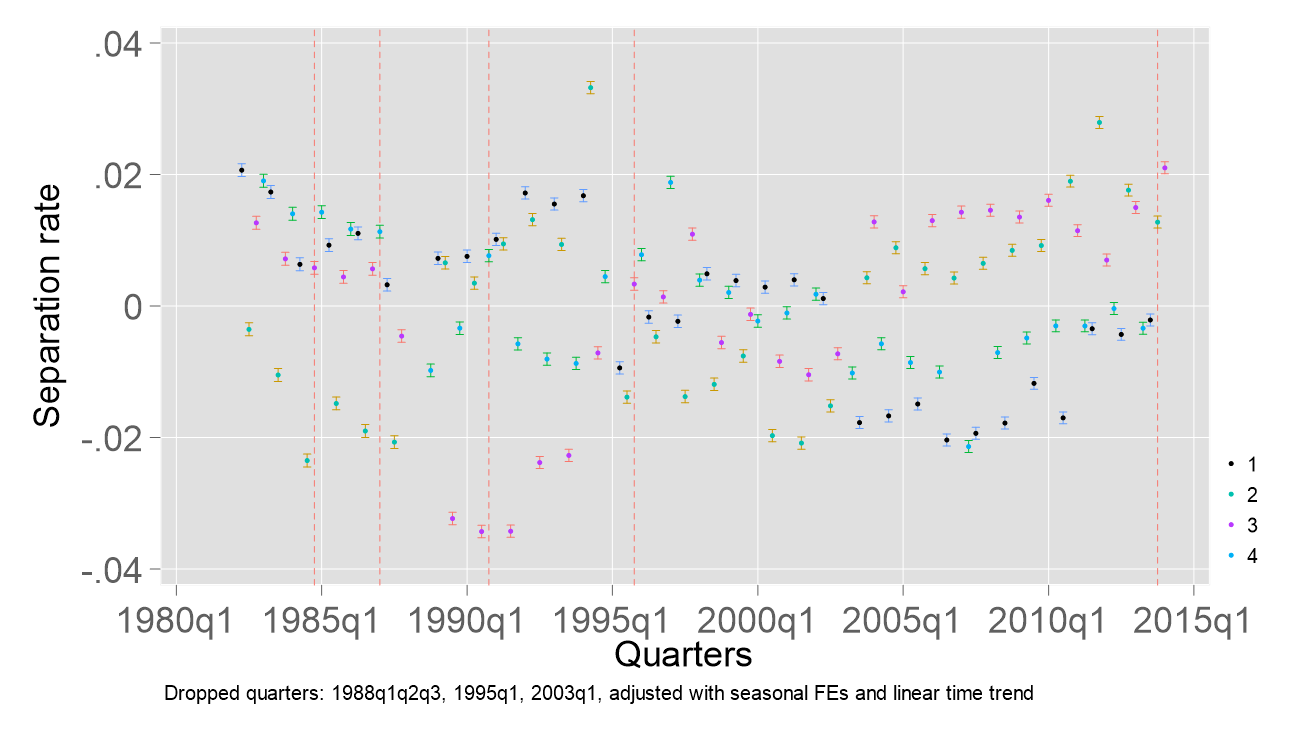
\includegraphics[width=0.9\textwidth]{../output/separation_rate_med_los.png}
    \end{figure}

\end{frame}

\begin{frame}
    \frametitle{Conclusions}

    \begin{wideitemize}
        \item In a first pass, there does not seem to be an obvious effect of shutdowns on the quality of who goes in and out of the federal government
        \item This holds for multiple measures of quality
        \item Government shutdowns are plausibly not as costly as one might fear from economic theory
    \end{wideitemize}
    
\end{frame}

\begin{frame}
    \frametitle{What is to be done}

    \begin{wideitemize}
        \item Triple diff design with departments treated and untreated (problem: around 1700 agencies, do not match easily)
        \item Double diff with just departments (same problem)
        \item Extending data possible, with loss of match quality after 2014
        \item Include DoD personnel, matching will be impossible after 2014
        \item Adding non-furlough shutdowns
        \item DiD design using our measures of quality
    \end{wideitemize}

\end{frame}

\begin{frame}
    \frametitle{}

    Appendix

\end{frame}

\begin{frame}
    \frametitle{Separation rates over time}

    \begin{figure}[]
        \centering
        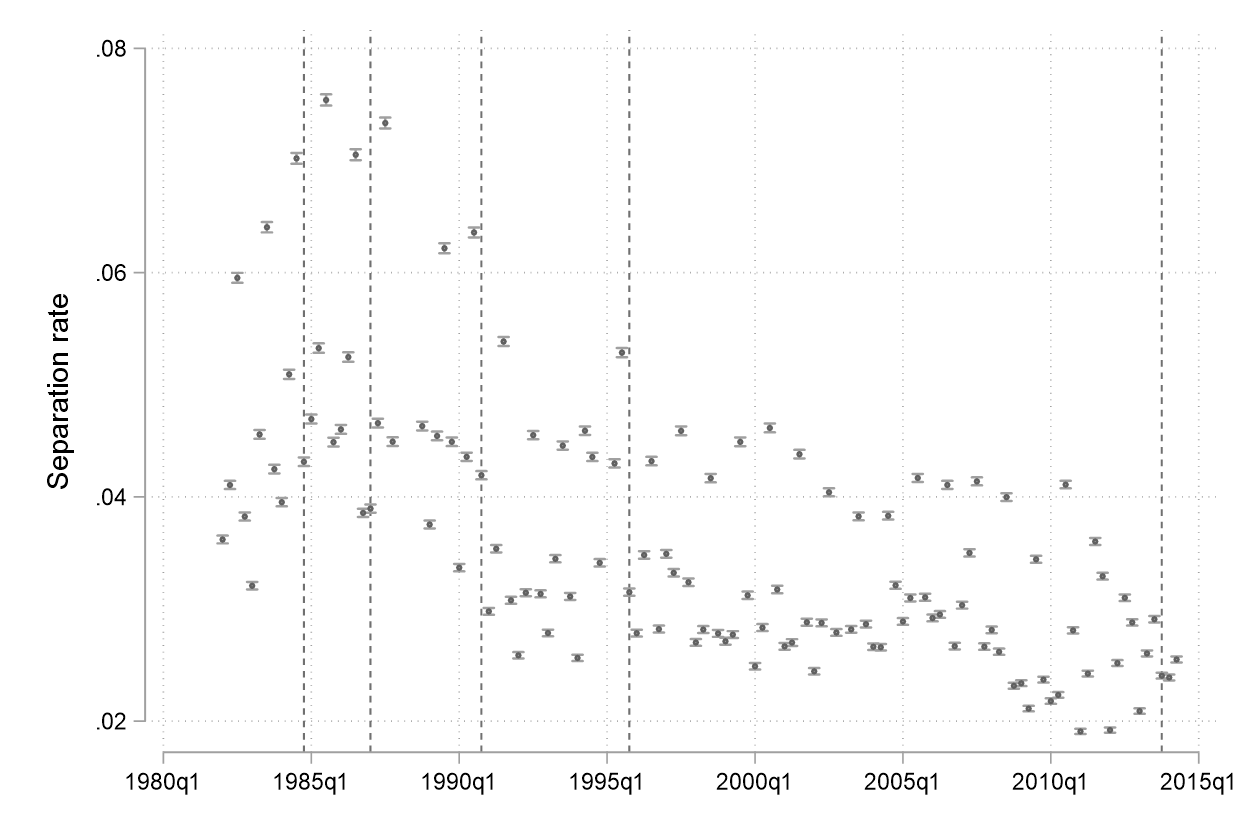
\includegraphics[width=0.9\textwidth]{../output/separation_rate_CI.png}
    \end{figure}

\end{frame}

\begin{frame}
    \frametitle{Accession rates over time}

    \begin{figure}[]
        \centering
        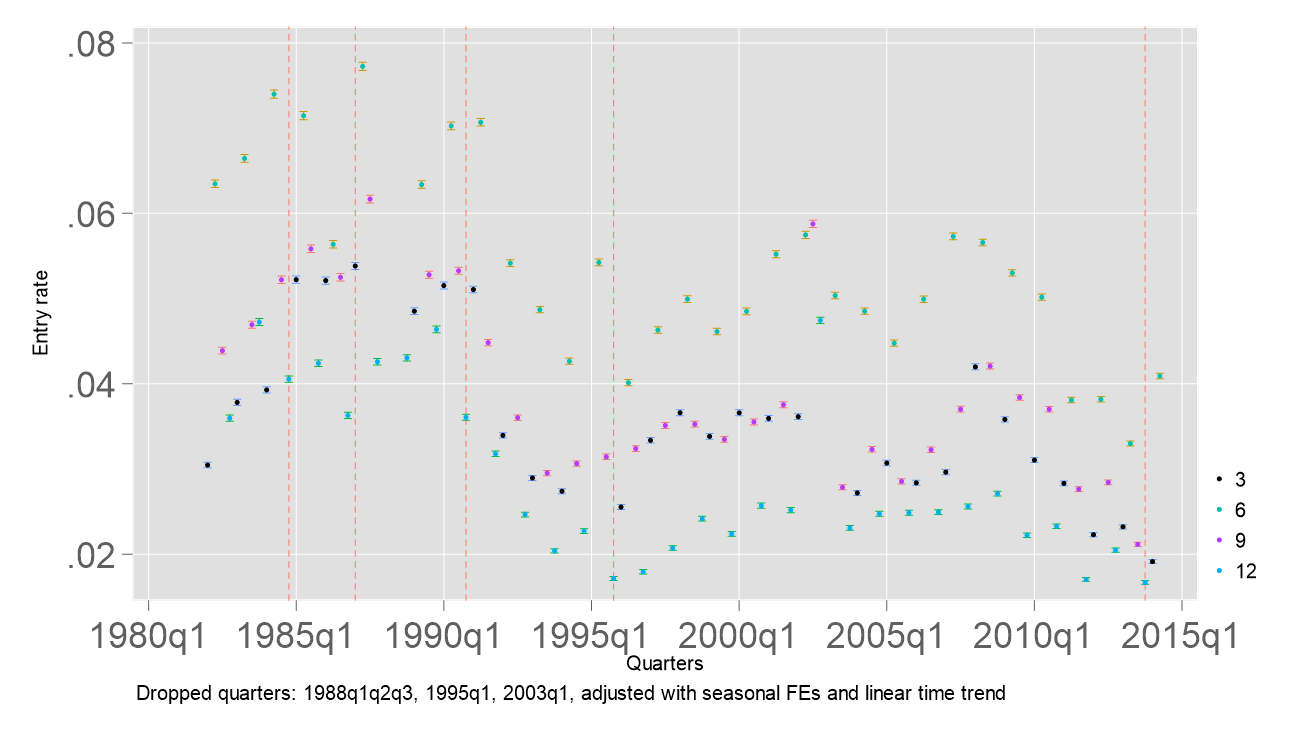
\includegraphics[width=0.9\textwidth]{../output/accession_rate_CI.png}
    \end{figure}

\end{frame}

\end{document}
